% =====================================================================
%  Query parser: SELECT-FROM-WHERE-GROUP BY-HAVING -> query block,
%  after [L14, s.6]
%  Compile:  pdflatex query-block.tex   (inside this folder)
%  Output:   query-block.pdf  -> 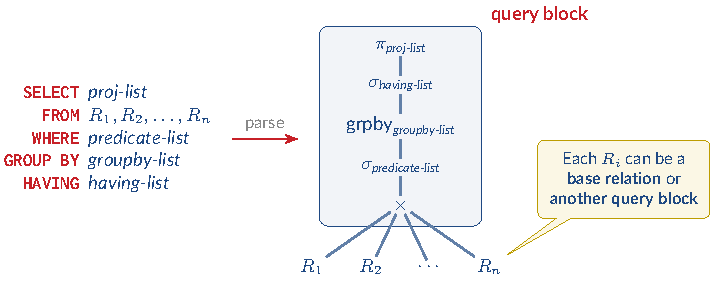
\includegraphics{query-block}
% =====================================================================
\makeatletter\def\input@path{{../../theme/}}\makeatother   % shared palette
\documentclass[tikz,border=2pt,11pt]{standalone}
\usepackage[T1]{fontenc}
\usepackage[defaultsans]{lato}
\usepackage[varqu,varl]{zi4}
\renewcommand{\familydefault}{\sfdefault}
\usepackage{amsmath}
\usepackage{vinuni-palette}
\usetikzlibrary{positioning,arrows.meta,fit,backgrounds,calc,shapes.callouts}

\newcommand{\kw}[1]{\textcolor{vinuRed}{\textbf{\ttfamily #1}}}
\newcommand{\ph}[1]{\textit{#1}}

\begin{document}
\begin{tikzpicture}[
    font=\footnotesize, text=vinuNavy,
    op/.style={inner sep=1.2pt, text=vinuNavy},
    link/.style={draw=vinuNavy!70, thick},
    node distance=3.2mm]

  % ---- SQL (left) ---------------------------------------------------
  \node[anchor=east, align=left, text=vinuNavy, inner sep=0] (sql) at (0,0) {%
    \begin{tabular}{@{}r@{\ \ }l@{}}
      \kw{SELECT}   & \ph{proj-list} \\
      \kw{FROM}     & $R_1, R_2, \ldots, R_n$ \\
      \kw{WHERE}    & \ph{predicate-list} \\
      \kw{GROUP BY} & \ph{groupby-list} \\
      \kw{HAVING}   & \ph{having-list}
    \end{tabular}};

  \draw[-{Stealth[length=2mm]}, thick, vinuRed] (0.35,0) -- node[above, font=\scriptsize, text=vinuGray] {parse} (1.45,0);

  % ---- query block (right): read bottom-up --------------------------
  \node[op] (pi)    at (3.2,1.55) {$\pi_{\textit{proj-list}}$};
  \node[op, below=of pi]    (hav)   {$\sigma_{\textit{having-list}}$};
  \node[op, below=of hav]   (grp)   {$\textsf{grpby}_{\textit{groupby-list}}$};
  \node[op, below=of grp]   (sel)   {$\sigma_{\textit{predicate-list}}$};
  \node[op, below=of sel]   (cross) {$\times$};
  \draw[link] (pi) -- (hav) -- (grp) -- (sel) -- (cross);

  \begin{scope}[on background layer]
    \node[draw=vinuNavy, fill=vinuNavy!6, rounded corners=1.5mm, inner xsep=4mm, inner ysep=2mm,
          fit=(pi)(hav)(grp)(sel)(cross)] (blk) {};
  \end{scope}
  \node[anchor=south west, font=\footnotesize\bfseries, text=vinuRed, inner sep=1pt]
    at ([xshift=1mm]blk.north east) {query block};

  % inputs of the cross product
  \node[op] (r1) at ($(cross)+(-1.5,-1.05)$) {$R_1$};
  \node[op] (r2) at ($(cross)+(-0.5,-1.05)$) {$R_2$};
  \node[op] (rd) at ($(cross)+( 0.5,-1.05)$) {$\cdots$};
  \node[op] (rn) at ($(cross)+( 1.5,-1.05)$) {$R_n$};
  \foreach \r in {r1,r2,rd,rn} \draw[link] (cross) -- (\r);

  % ---- callout ------------------------------------------------------
  \node[rectangle callout, draw=vinuGold!90!black, fill=vinuGold!10, rounded corners=1mm,
        align=center, font=\scriptsize, text=vinuNavy, inner sep=2mm,
        callout absolute pointer={(rn.north east)}]
    at ($(blk.east)+(2.4,-0.9)$) {Each $R_i$ can be a\\ \textbf{base relation} or\\ \textbf{another query block}};
\end{tikzpicture}
\end{document}
